\section{Brownian motion on an ARG} %Methods

%

% To infer dispersal rates and ancestral locations, we first assume that we have access to a time-calibrated ARG with recombination nodes (often referred to as a ``full" ARG, e.g., \cite{Baumdicker2022,shipilina2023origin,lewanski2023era}). 

An ARG is a graphical representation of the genealogical history of a set of sample genomes that may have undergone recombination in the past \citep{Wong2023}. As the history of the samples at each site in the genome can be depicted as a tree, an ARG weaves together these histories based upon their shared structure. Altogether, an ARG provides the complete genetic history of the samples across the chromosome. Each node in an ARG represents a haploid genome. Edges are directed from an ancestral node to a descendant node, describing the line of inheritance over time. A node that is the product of recombination has two ancestral nodes with annotated edges referring to the specific regions of the chromosome that were inherited from each. Time is measured backwards from the present, starting from the most recent sample node at time $t=0$ and increasing as we go deeper into the past towards the root of the ARG, i.e. its gMRCA, grand most recent common ancestor \citep{Wong2023}. In this work we focus on "full ARGs", which include the complete set of coalescent, recombination, and common ancestor nodes. This is mainly for ease of explanation. %acknowledging that some of these nodes may be "unknowable" outside of a theoretical context. 
Our conclusions and algorithms are applicable more broadly to commonly inferred "simplified ARGs", which only include coalescent nodes found in the local trees \citep{Wong2023,Baumdicker2022,shipilina2023origin,lewanski2023era}.

%An ARG is graphical representation of the genealogical history of a set of sample genomes that may have undergone recombination in the past \citep{Wong2023}. As the history of the samples at each site can be depicted as a tree, an ARG weaves together these histories based upon their shared structure to represent the history of the samples across the entire genome. Each node in an ARG represents a haploid genome and directed edges connect these nodes to describe the line of inheritance over time. Nodes that are the product of recombination will be connected to two ancestral nodes with annotated edges referring to the specific regions of the chromosome that were inherited from each ancestor. Here, we define a path through the ARG as a sequence of edges which connects a sample node (a tip of the ARG) back in time to a root. Time is measured backwards from the present, starting from the most recent sample node at time $t=0$ and increasing as we go deeper into the past towards the root(s).

We model the movement of genetic material forward in time by Brownian motion with dispersal rate $\sigma^2$ (see Table \ref{table:methods} for a list of key symbols). In other words, we assume that the location of a node is normally distributed about its parent node with variance $\sigma^2 t$, where $t$ is the length of the edge connecting them (in generations). In each generation, autosomal inheritance is equally likely via the mother or father; therefore, the effective variance is the average of maternal and paternal variances \citep[e.g., see][]{smith2023dispersal}. While the computations are shown for one dimension, they are readily extended to two dimensions by replacing the dispersal rate, $\sigma^2$, with a dispersal matrix, $\Sigma = \begin{bmatrix} 
    \sigma_x^2 & \sigma_{xy} \\
    \sigma_{xy} & \sigma_y^2
\end{bmatrix}$. We assume we know the ARG with certainty and therefore all edges are treated equally regardless of the amount of chromosome they span; if we know with certainty that an edge exists in the graph, the span is of no influence. This differs from the approach of \cite{grundler2024}, which gives less weight to edges with smaller spans due to the lower confidence in accurately inferring these short span edges from genetic data. Here we are focused on developing theory rather than applying a method.

\begin{table}
\caption{Description of key symbols used}
\begin{center}
\begin{tabular}{ | m{3.5em}|m{9em}|m{20em}| } 
 \hline
 Symbol & Name & Description and Notes \\ 
 \hline
 $n_s$ & Number of samples &  \\ 
 \hline
 $n_p$ & Number of paths & Total number of paths from all samples to the root \\ 
 \hline
 $n_r$ & Number of roots & Total number of roots in the ARG \\ 
 \hline
 $\sigma^2$ & Dispersal rate & Variance in the offspring locations relative to parent location \\ 
 \hline
 $\spath$ & Path Matrix & Entries are shared times between any two paths. This could refer to either the Full Path Matrix of the Minimal Path Matrix  \\
 \hline
 $\mathbf{S}$ & Sample Matrix & $\sigma^2 \mathbf{S}$ is covariance matrix between sample locations \\ 
 \hline
 $\Pp$ & Path-Sample Matrix & $n_p \times n_s$ matrix whose entry is 1 if path $i$ is associated with sample $j$ \\ 
 \hline
 $\Rp$ & Path-Root Matrix & $n_p \times n_r$ matrix whose entry is 1 if path $i$ is associated with root $j$ \\ 
 \hline
 $\Lvec$ & Sample location vector & Vector valued random variable of sample locations of length $n_s$  \\ 
 \hline
 $\Lpvec$ & Path location vector &  Vector valued random variable of length $n_p$\\ 
 \hline
 $\muvec$ & Root location vector &  Vector of length $n_r$\\ 
 \hline
 $\Lint$ & Internal node location & Random variable denoting location of internal node $a$\\ 
 \hline
 $\savec$ &  & Vector valued random variable of length $n_p$ with shared time between the path of internal node $a$ and paths corresponding to $\spath$ \\ 
 \hline
 $V$ & Ancestor specific uncertainty & Component of location variance related to ancestor timing and root uncertainty \\
 \hline
\end{tabular}
\label{table:methods}
\end{center}
\end{table}


% \begin{table}[ht]
% \caption{Description of key symbols used}
% \begin{center}
% \begin{tabular}{ | m{3.5em}|m{9em}|m{20em}| } 
%  \hline
%  Symbol & Name & Description and Notes \\ 
%  \hline
%  $s$ & Number of samples &  \\ 
%  \hline
%  $p$ & Number of paths & Total number of paths from all samples to the root \\ 
%  \hline
%  $r$ & Number of roots & Total number of roots in the ARG \\ 
%  \hline
%  $\sigma^2$ & Dispersal rate & Variance in the offspring locations relative to parent location \\ 
%  \hline
%  $\mathbf{S}_p$ & Path Matrix & Entries are shared times between any two paths. This could refer to either the Full Path Matrix of the Minimal Path Matrix  \\ 
%  \hline
%  $\mathbf{S}$ & Sample Matrix & $\sigma^2 \mathbf{S}$ is covariance matrix between sample locations \\ 
%  \hline
%  $\mathbf{P}$ & Path-Sample Matrix & $p \times s$ matrix whose entry is 1 if path $i$ is associated with sample $j$ \\ 
%  \hline
%  $\mathbf{R}$ & Path-Root Matrix & $p \times r$ matrix whose entry is 1 if path $i$ is associated with root $j$ \\ 
%  \hline
%  $\Lvec$ & Sample location vector & Vector valued random variable of sample locations of length $s$  \\ 
%  \hline
%  $\Lpvec$ & Path location vector &  Vector valued random variable of length $n_p$\\ 
%  \hline
%  $\muvec$ & Root location vector &  Vector of length $r$\\ 
%  \hline
%  $\Lint$ & Internal node location & Random variable denoting location of internal node $a$\\ 
%  \hline
%  $\savec$ &  & Vector valued random variable of length $p$ with shared time between the path of internal node $a$ and paths corresponding to $\spath$ \\ 
%  \hline
% \end{tabular}
% \label{table:methods}
% \end{center}
% \end{table}





%Brownian motion is a commonly used model in phylogeography \citep[e.g.,][]{lemmon2008likelihood}, where there is a single tree relating the samples, directly analogous to earlier models of continuous trait evolution on a phylogeny \citep{Felsenstein1985}. More recently, this model has been applied to sets of trees sparsely sampled along the genome \citep{Osmond2021} assuming independence between each sampled tree. As we explain below, extending this approach from a sequence of independent trees to a graph is non-trivial. We will start by building intuition through the simplest examples, such as small, handmade ARGs with a single root, before tackling more complex scenarios that arise from simulations. While all samples are contemporary in the ARGs presented in this paper ($t=0$), our method can be readily used with non-contemporary samples, including samples that are direct ancestors of another sample.

%\subsection{Problem of Loops}

%There are many examples of applying Brownian motion to individual trees [CITE THESE PAPERS].

All of the equations presented here are generalizations of the standard tree-based approach to account for recombination. As a tree is simply an ARG without recombination, these generalized equations will all collapse back to those previously presented in literature for a single tree.

The first step in estimating dispersal rates and the locations of genetic ancestors given an ARG is calculating a likelihood for the sample locations. Under Brownian motion, the vector of sample locations, $\Lvec$, has a multivariate normal distribution, specifically,
%
\begin{eqnarray}\label{eqn:Lvec}
    \Lvec \sim \cN(\mu \onevec{{n_s}},\sigma^2 \mathbf{S} ),
\end{eqnarray}
%
where $\mu$ is the location of the root (gMRCA) of the ARG, $\onevec{{n_s}}$ is a column vector of length $n_s$ (number of samples) consisting of just ones, $\sigma^2$ is effective the dispersal rate, and $\sigma^2 \mathbf{S}$ is the covariance matrix between the sample locations. We refer to $\mathbf{S}$ as the "sample matrix" and it represents the covariance between the samples that is solely due to the structure of the ARG, independent of the dispersal rate. The entries of this sample matrix, $\mathbf{S}$, for a tree are simply the shared times between each pair of sample paths. For an ARG, this matrix is not straightforward to compute (reasons explained below) but it is the key to computing the maximum likelihood estimates (MLEs) of the root location, $\mu$, and the dispersal rate, $\sigma^2$.

For a single tree, we can assume that the displacement along any edge is independent of the other edges' displacements. The displacement of an edge from node $i$ to node $j$ is distributed as $D_{i,j} \sim \cN(0,\sigma^2 t_{i,j})$, where $t_{i,j}$ is the length of the edge in generations. The sample's location is given by the sum of the displacements along the edges from the root to the sample. We refer to a series of edges connecting an older (further in the past) node to a more recent node as a "path". We are particularly interested in paths from the root to a sample and call the set of such paths the "sample paths". The covariance between the locations of two samples is then simply $\sigma^2$ times the shared time between the unqiue corresponding sample paths, hence the entries of $\mathbf{S}$ are just the shared time between each pair of samples, as mentioned above. 

In generalizing this approach to an ARG we run into two related issues. First, each recombination node creates a loop within the graph. This means that samples found below a recombination node will have multiple paths back to the root. Therefore, computing the entries of $\mathbf{S}$ for an ARG is not as straightforward as it is for a tree and the covariance between samples must take into account this braided history where multiple paths lead to the same sample. Second, the presence of these loops means that we can no longer always assume that the displacements along edges of the graph forward in time are independent. Assuming that the parents of a recombination node must precisely meet each other in space, the displacement along the edges involved in the loop must satisfy the condition that the sum of the displacements around the left half of the loop equal the sum around the right half. For example, in Figure \ref{fig:method} the displacement from node $G$ to node $F$ plus the displacement from node $F$ to node $E$ must equal the displacement from node $G$ directly to node $E$, $D_{G,F} + D_{F,E} = D_{G,E}$. We refer to the collection of these conditions across an ARG as $\eta_\mathrm{loops}$.

\begin{figure}[H]
    % \centering
    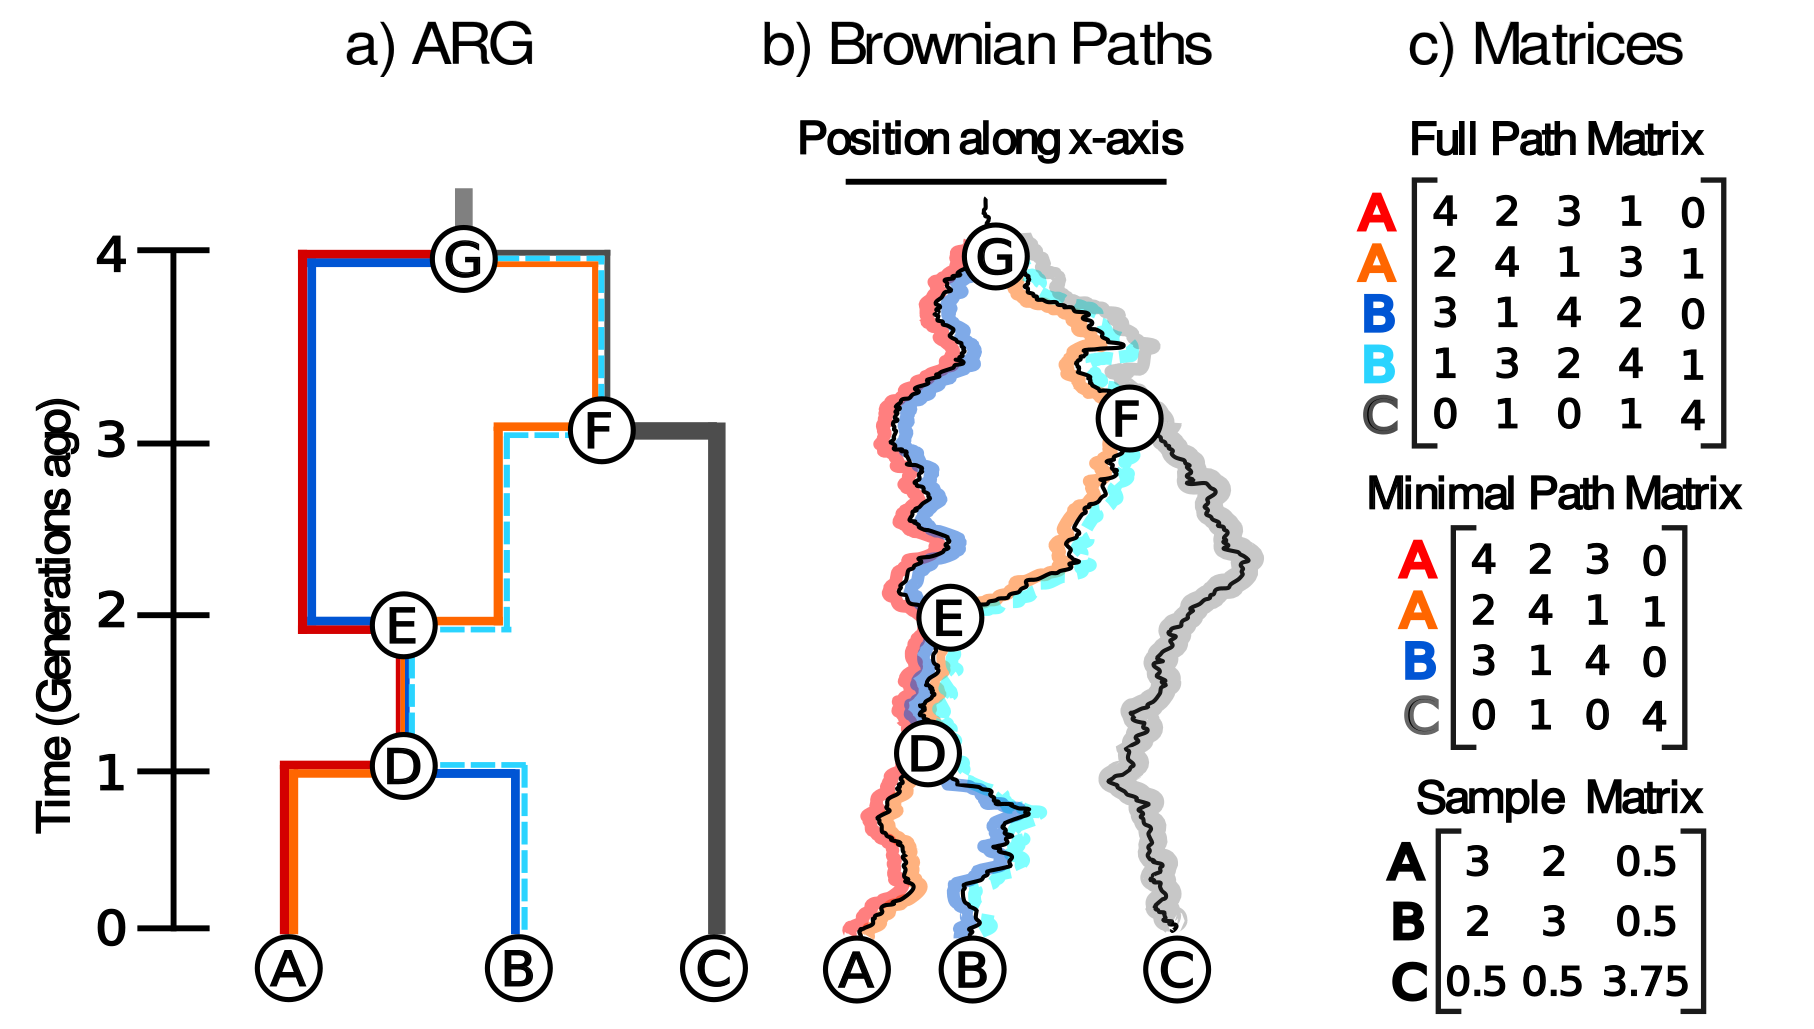
\includegraphics[width=\linewidth]{Images/Figure1_Method/Fig1_Method_Simplified.png}
    \caption{\textbf{Brownian motion on an ARG.} (a) An ARG, (b) an instance of Brownian motion along the ARG, and (c) the corresponding path and sample matrices. Sample paths through the ARG are individually colored. Samples $A$ and $B$ are associated with two paths each - red/orange and navy/sky blue, respectively - because they are beneath a recombination node (node $E$). In the Brownian motion model illustration, note that the paths meet precisely at the recombination node $E$. The path matrices contain the shared time between the sample paths. The sky blue path from sample B is excluded when calculating the minimal path matrix as it provides redundant information.}%Overview of methods. (A) A simple example ARG of three samples with sample paths highlighted in different colors. The dashed blue line is the sample path that is excluded while calculating the minimal path matrix. (B) A cartoon of Brownian motion down this ARG. Note that we are implicitly assuming here that the lineages all coalesce in the recent past, otherwise their spatial locations would traverse back and forth across space instead of neatly merging to the middle. (C) The full and minimal path matrices and the corresponding sample matrix. (D) Illustration of the bottom-up algorithm to build the minimal path matrix.}
    \label{fig:method}
\end{figure}

% \subsection{The path matrix}

To account for these additional conditions, $\eta_\mathrm{loops}$, we start by assuming (incorrectly) that Brownian motion along each edge of the ARG is indeed independent, as in the case of trees. This leads to the same sample node having different location distributions based on the choice of sample path. Nevertheless, we encode the distribution of locations of the nodes at the tips of each sample path in $\Lpvec$, a column vector of length $n_p$ (number of sample paths) with distribution 
%
\begin{eqnarray}\label{eqn:Lvec_paths}
    \Lpvec \sim \cN(\mu \onevec{{n_p}},\sigma^2 \spath),
\end{eqnarray}
%
where $\spath$, referred to as the path matrix, is the matrix of shared times between sample paths. To get the correct distribution of sample locations, $\Lvec$ (Equation \ref{eqn:Lvec}), we need to condition $\Lpvec$ so that all sample paths that end at the same sample also end at the same location. We refer to this condition as $\eta_\mathrm{paths}$ and show that $\eta_\mathrm{paths}$ reduces to $\eta_\mathrm{loops}$ (Appendix \ref{appendix:Equivalence}). The sample matrix can then be easily computed from the path matrix (Appendix \ref{appendix:MLE}),
%
\begin{eqnarray}
  \mathbf{S} = (\Pp^T\spathg\Pp)^{-1}.
  \label{eqn:S}
\end{eqnarray}
%
Here, $\spathg$ is the generalized inverse of $\spath$ and $\Pp$ is a conversion matrix of size $n_p \times n_s$ that pairs each sample path $i$ with its associated sample $j$. The $i,j^{th}$ element of $\Pp$ is 1 if path $j$ starts at sample $i$, otherwise it is 0. As a check, note that the sample matrix and path matrix are equivalent for a tree (i.e., when there is no recombination) as each sample is associated with only one path. 

We can now compute the likelihood of sample locations (Equation \ref{eqn:Lvec}). Though this conversion from $\spath$ to $\mathbf{S}$ is possible, it is generally unnecessary and it is anyways easier to work with the path matrix in what follows. 
Additionally, while we could calculate the shared times between every pair of sample paths through the ARG, many of the paths are not linearly independent from one another and are therefore redundant in our calculations. In practice, we use only a minimal subset of paths and its corresponding minimal path matrix (see Figure \ref{fig:method} for an example). While the total number of sample paths grows faster than linearly with the number of recombination events, the minimal number of sample paths grows linearly (being equal to the number of samples plus the number of recombination events; see Appendix \ref{appendixC:description}). We have developed an algorithm to calculate the minimal path matrix in a single tip-to-root traversal of the ARG (Appendix \ref{appendixC}).


%The methods for calculating $\mathbf{S}$ differ when working with trees versus ARGs. In the case of a tree, we can assume that the displacement along any edge of the tree forward in time is independent of the displacement along every other edge and is distributed as $D_{edge} \sim \cN(0,\sigma^2 t_{edge})$, where $t_{edge}$ is the length of the edge. We define a path through the ARG as a sequence of edges which connects a node back in time to a root. In a tree, each sample is associated with a single path. Hence, the sample location is given by the sum of the displacements along all edges in the sample's path. The entries of the sample matrix, $\mathbf{S}$, for a tree are then simply the shared times between the paths associated with the corresponding pair of samples. Computing the entries of $\mathbf{S}$ for an ARG is not as straightforward because of two related reasons stemming from the presence of recombination nodes. Firstly, each recombination node creates a loop within the graph. We assume that two individuals have to physically be at the same location for mating, so the two parental lineages need to meet at the recombination node. The displacement along the edges involved in the loop are not independent; they must satisfy the condition that the sum of the displacements around the left half of the loop must equal the sum around the right half. For instance in Figure \ref{fig:method}, the displacement from node 7 to node 6 and the displacement from node 6 to node 4/5 must sum to the displacement from node 7 directly to node 4/5,  $D_{7,6} + D_{6,4/5} = D_{7,4/5}$. Each recombination node in a graph has an associated loop, and we define $\eta_\mathrm{loops}$ as the combination of all of these constraints. Secondly, the presence of a loop means that the samples below the recombination node have multiple paths connecting them to the same root. For example in Figure \ref{fig:method}, there are two paths that connect sample $0$ to the root, $(0,3,5,6,7)$ and $(0,3,4,7)$. It is therefore not possible to calculate a single shared time between two samples, as it was for a tree.



%\subsection{Solution of Paths}

%To solve this problem, we start by incorrectly allowing the displacement along each edge in the ARG to be independent. This means that a sample with multiple paths to the root has multiple locations, one for each path. Let $n_p$ be the total number of paths from all the samples to the root. Unlike trees, where the number of paths is always equal to the number of samples, the number of paths through an ARG grows with the number of recombination nodes within the graph. Let $\Lpvec$ be a vector of length $n_p$ containing the sample locations of each of these paths. $\Lpvec$ is then multivariate normal with mean $\mu \onevec{p}$ and covariance matrix $\sigma^2 \spath$, where $\spath$ is the matrix of shared times between each pair of paths. In order to compute the correct distribution of the sample locations, $\Lvec$, we need to condition $\Lpvec$ on the paths along the same recombination loop meeting, $\eta_\mathrm{loops}$. While computing $\Lpvec | \eta_\mathrm{loops}$ is possible, it is cumbersome and difficult to do algorithmically. Instead, we condition on an equivalent set of events, that all paths starting at the same sample should have the same location. We call this set of events $\eta_\mathrm{paths}$. In Figure \ref{fig:method}, this set consists of two conditions, one corresponding to paths ending at sample $0$ and the other at sample $1$, $\eta_\mathrm{paths} = \{ \mu + D_{7,4/5} + D_{4/5,3} + D_{3,0} = \mu + D_{7,6} +D_{6,4/5} + D_{4/5,3} + D_{3,0} \ , \ \mu + D_{7,4/5} + D_{4/5,3} + D_{3,1} = \mu + D_{7,6} +D_{6,4/5} + D_{4/5,3} + D_{3,1} \}$. Note that by canceling common terms on opposite sides of the equality, $\eta_\mathrm{paths}$ reduces to  $\eta_\mathrm{loops}$, which we can prove more generally (Appendix \ref{appendix:Equivalence}). $\Lpvec | \eta_\mathrm{paths}$ is easier to compute algorithmically and gives the same normal distribution as above (Equation \ref{eqn:Lvec}), with the sample covariance matrix now defined as 

%\begin{eqnarray}
%  \mathbf{S} = (\Pp^T\spathg\Pp)^{-1}.
%  \label{eqn:S}
%\end{eqnarray}

%Here, $\spathg$ is the generalized inverse of $\spath$ and $\Pp$ is a conversion matrix of size $n_p \times n_s$ that pairs each path $i$ with its associated sample $j$ (see Appendix \ref{appendix:MLE} for a proof). The $i,j^{th}$ element of $\Pp$ is 1 if path $j$ starts at sample $i$, otherwise it is 0.

%Finally, while we could calculate the shared times between every path through the ARG, many of the paths are not linearly independent from one another and are therefore redundant in our calculations. In practice, we use only a minimal subset of paths and its corresponding shared time matrix (see Figure \ref{fig:method} for an example). While the total number of paths grows rapidly (faster than linearly) with the number of recombinations, the minimal number of paths grows linearly (being equal to the number of samples plus the number of recombinations; see Appendix \ref{appendixC:description}).

\subsection{Multiple roots}

There are many reasons why we might want to focus on just the recent past. First, long-term movement may not be accurately captured by Brownian motion due to geographic boundaries or large-scale population movements \citep{Ianni2022}. Second, as we move further back into the past, sample lineages can become spatially well mixed \citep{Wakeley1999}, which makes it difficult or impossible to extract meaningful spatial information about the deep history of samples. Third, with ARG inference, deeper nodes in the ARG are often poorly resolved, both in timing and topology (CITE). To avoid these issues, we will often want to cut off an ARG at a given time in the past and ignore any deeper connections.

When we chop an ARG below the grand most recent common ancestor (root), the graph no longer has a single root (Figure \ref{fig:MultipleRoots}). Instead there are multiple roots, each being associated with specific paths through the ARG. Let $\muvec$ be the vector of root locations (of length $n_r$, the number of roots) and $\Rp$ be a conversion matrix of size $n_p \times n_r$. The $i,j^{th}$ element of $\Rp$ is 1 if path $j$ terminates at root $i$, otherwise it is 0. Then $\Rp \muvec$ is the vector of root locations associated with each of the $n_p$ paths.

The full covariance between the locations of the ends of the sample paths is the covariance created by the structure of the ARG plus the covariance between the root locations, $\sigma^2 ( \spath + \text{Cov}(\Rp\muvec, \Rp\muvec))$. Here, we assume that the root locations are independent of each other and that each has zero variance, $\text{Cov}(\Rp\muvec, \Rp\muvec)=0$, so that the covariance between the locations of the ends of the sample paths remains $\sigma^2 \spath$. The assumption of independence is reasonable if we cut off the ARG at a point by which the ancestors are well mixed in a finite habitat. The assumption of zero variance in root locations can be relaxed by adding a variance to the covariance term between pairs of paths starting at the same root.

\textcolor{red}{i think we should end here with our eqn for distn of sample locations with multiple roots, which i think is just eqn 1 with $\mu$ updated by $\Rp$?}

\subsection{Estimates}

If $\Rp^\text{T}\spathg\Rp$ is invertible, we can compute the MLEs for the root locations given the observed sample locations, $\ldata$, as the unique solution to (Appendix \ref{appendix:MultipleRoots})
%
\begin{eqnarray}
 \muvecMLE = (\Rp^\text{T}\spathg\Rp)^{-1} \Rp\spathg\Pp\ldata.   
\end{eqnarray}

% We can compute the MLEs for the root locations given the observed sample locations, $\ldata$, as a solution to 
% \begin{eqnarray}
%     \label{eq:location_of_roots}
%     \Rp^\text{T}\spathg\Rp  \muvecMLE = \Rp\spathg\Pp\ldata  
% \end{eqnarray}
% (see Appendix \ref{appendix:MultipleRoots} for a proof). If $\Rp^\text{T}\spathg\Rp$ is invertible, then there exists a unique solution,
% \begin{eqnarray}
%  \muvecMLE = (\Rp^\text{T}\spathg\Rp)^{-1} \Rp\spathg\Pp\ldata.   
% \end{eqnarray}

% \subsection{Dispersal Rate and Location of Genetic Ancestors}

Once we have estimated the locations of the roots, we can compute the MLE of the dispersal rate,
\begin{eqnarray}\label{eq:sigmaMLE}
    \sigmaMLE &=& \displaystyle \frac{ (\Pp\ldata - \Rp\muvecMLE)^\text{T} \spathg (\Pp\ldata - \Rp\muvecMLE) }{n_s}.
\end{eqnarray}

With estimates of both the root locations and the dispersal rate, we can then calculate the distribution of any internal node location (a genetic ancestor). Given an internal node, we choose an arbitrary path from that node to one of the roots. Conditional on the dispersal rate, root locations, and observed sample locations, the location of an internal node, $L_a$, is normally distributed with mean
\begin{eqnarray}\label{eq:Lint}
    E[\Lint | \muvecMLE, \sigmaMLE] =  \muMLE_{r_a} + \savec^\text{T}\spathg(\Pp\ldata - \Rp \muvecMLE),
\end{eqnarray} 
where $\savec$ is the vector of shared times with the minimal paths used to construct $\spath$ and $\muMLE_{r_a}$ is the MLE location of the $r_a$\textsuperscript{th} root (the $r_a$\textsuperscript{th} element of $\muvec$). 
The total variance in the internal node's location is a combination of the variance due to Brownian motion and the variance due to uncertainty in the root locations,
%\begin{eqnarray}\label{eq:VarLint}
%    \Var (\Lint) = \sigmaMLE\bigg(\underbrace{t_a - \savec^\text{T}\spathg\savec}_{\text{due to Brownian motion}} + \ \ \underbrace{(\vec{e}_{r_a} - \Rp^\text{T}\spathg\savec)^\text{T} ( \Rp^\text{T}\spathg\Rp )^{-1} (\vec{e}_{r_a} - \Rp^\text{T}\spathg\savec)}_{\text{due to uncertainty in root locations}}    \bigg), 
%\end{eqnarray}
\begin{eqnarray}\label{eq:VarLint}
    \Var (\Lint) = \sigmaMLE V,
\end{eqnarray}
where
\begin{eqnarray}\label{eq:ancestor_specifc_uncertainty}
    V = \underbrace{t_a - \savec^\text{T}\spathg\savec}_{\text{due to Brownian motion}} + \ \ \underbrace{(\vec{e}_{r_a} - \Rp^\text{T}\spathg\savec)^\text{T} ( \Rp^\text{T}\spathg\Rp )^{-1} (\vec{e}_{r_a} - \Rp^\text{T}\spathg\savec)}_{\text{due to uncertainty in root locations}}, 
\end{eqnarray}
and $\vec{e}_{r_a}$ is a length $n_r$ column vector that is zero everywhere except with a 1 at the $r_a$\textsuperscript{th} position. 

% We break down the location variance into its two major components: the dispersal rate estimate for the ARG and the uncertainty specific to the ancestor in question. In the following sections, we've found it helpful to discuss these components of the variance separately as bias in dispersal rate estimates (described in Section \ref{dispersal_rate_section}) often masks the behavior of the ancestor specific uncertainty ($V$).

%\subsection{Algorithm}

%The key object for estimating dispersal rates and ancestor locations is the matrix of shared times between the minimal set of paths through the ARG, $\spath$. Though there are existing methods in {\tt Python} to identify all paths from the samples to the roots, calculating the intersection between these paths does not scale well to larger ARGs, primarily due to repeated calculation of common edges across different paths (Figure \ref{fig:algo_and_bench}). We therefore developed an algorithm that requires traversing each edge only once (Appendix \ref{appendixC}) and, in doing so, have greatly sped up the calculation of $\spath$ (Figure \ref{fig:algo_and_bench}). 

%\begin{figure}[hbtp]
    % \centering
    %\includegraphics[width=\linewidth]{Image/Fig2_AlgoBench.png}
    %\caption{\textbf{Algorithm benchmarks}. Number of seconds to compute the full path and minimal path matrices using different algorithms plotted as a function of the total number of paths in the ARG. ``Full Path Matrix - Naive" (blue) uses existing Python methods to compute the full path matrix. ``Full Path Matrix - Bottom up" (red) instead computes the full path matrix with a single bottom-up traversal of the ARG. ``Minimal Path Matrix" (orange) uses the bottom-up method to compute the covariance between the smallest set of linearly independent paths, which is sufficient for estimating parameters of interest. Random ARGs of various sizes were generated (number of samples ranged up to 500 and sequence lengths up to 5000 basepairs) using the msprime Python package. The solid lines are the best fits under a power law. The best fit exponents for the power law are 2.946 (Full Path - Naive), 1.432 (Full Path - Bottom up) and 0.853 (Minimal Path).}
    %\label{fig:algo_and_bench}
%\end{figure}

%Briefly, the algorithm entails a bottom-up traversal of the ARG starting at the sample nodes and updating the shared time matrix as we move upwards towards the roots (Figure \ref{fig:algo_and_bench}). For each node visited, the algorithm calculates the edge length between that node and its parent. This is added to the corresponding cells in the shared time matrix. When we reach a recombination node (which has multiple parents), the relevant rows and columns are duplicated, expanding the size of the matrix and corresponding with the separation of these paths in the ARG. This keeps the size of the matrix small for as long as possible, making it more efficient. Currently, the algorithm is implemented using the {\tt tskit} package \citep{Kelleher2018}.

%\subsection{Windowing}

%While our method and algorithm are designed to scale to full chromosomes, we can decide to analyze a smaller portion (window) of the genome, e.g., a window centered on a particular locus or the recombination breakpoint of interest. Windowing may also offer a more practical approach when working with large datasets, such as biobanks \citep[e.g.,][]{zhang2023biobank}. 

%There are number of ways we can choose windows. A genetic ancestor (internal node) is associated with a specific region of the chromosome. To locate this ancestor we may therefore want to center a window at the center of this region, which will generally fall within a local tree. The smallest window we can consider is simply this local tree. In contrast, we might be interested in a particular recombination event, which necessarily falls directly between two local trees. The smallest window we then want to consider is the two neighboring trees. Here, we define the size of a window as the number of neighboring trees on either side of the smallest window. This means that a window of size 0, referred to in the results as $W_0$, includes just the windows described above (local tree for genetic ancestor or two neighboring trees for recombination breakpoint). A window of size 1 ($W_1$) includes one neighboring tree on either side of the smallest interval, and so on. When a window extends beyond an edge of a chromosome there will be fewer trees than the window size suggests. Smaller windows are faster to analyze  but contain less information. The size of a suitable window will likely depend on the organism and sample, and remains an open question. Note that different windows will give different locations for the same node.

% Importantly, setting the window size based on the number of neighboring trees generally results in windows being of different sequence lengths (Figure \ref{fig:WindowSizeDistributions}); the structure of the ARG is unaffected by the sequence length that each tree spans, only the number of trees included. 

% Each genetic ancestor is centered within its own window and associated trimmed ARG; this means that the shared time matrix will differ when estimating the locations of genetic ancestors that are centered on different trees. In its current implementation, we avoid redundant calculations by first checking if there are any perfectly overlapping windows across the genetic ancestors that can use the same ARG calculations. 

%\subsection{Alternative Brownian Motion model}
%There are multiple ways of modeling Brownian dispersal over a network. Particularly, there are choices to be made about what happens at a recombination node. In our model, we necessitate that two parent lineages meet (forward in time) at the recombination node. However, it is known that meeting of two Brownian lineages is very low, hence conditioning on it is a strong requirement. Further, in reality, the parents can don't need to be at the exact same location, for instance pollen dispersal in plants can allow mating between individuals located far apart. Further, even when mating require physical proximity, it is possible that individuals can identify mates from far away due to sensory calls (mating calls and visual cues etc.). Once the mate location is identified, the movement of the individual is directed towards that location and is no longer random. Therefore, the Brownian only needs to get the mates within some distance of each other. We explore the extreme version of this relaxed Brownian model, where the parents can be arbitrarily far from each other and the offspring is placed at the midpoint of their locations. The covariance matrix for this model has been computed previously (in \cite{Bastide2018}) and can be obtained from our Full Paths Matrix (see Appendix \ref{appendix:RelaxedBM}). % 

%\section{Spatially-Explicit Simulations}

%To assess the utility of our method to infer parameters under more realistic dynamics than Brownian motion, we simulate density-dependent reproduction as well as finite boundary habitats. Simulations started with 10,000 individuals uniformly randomly distributed in a $100 \times 100$ unit area, with each individual being diploid for a 1 megabase chromosome.  All individuals are hermaphrodites. In each generation an individual acts once as a mother, choosing its mate randomly based on distance (we assume a Gaussian mating kernel with variance $\sigma^2_m$). The number of offspring for each mating pair is a Poisson random variable with mean $\lambda=\frac{2}{1 + C}$, where C is the sum of the interaction strengths with neighbors. Here, interaction strengths are Gaussian with variance $\sigma^2_c$. It is possible that there are no mates within the interaction distance, in which case no offspring are produced. Offspring are placed relative to their mother's position with a normal random variable offset in each dimension with variance $\sigma^2_d$. If the offset would place the offspring outside of the area, the offset is reflected off of the boundary wall and back into the area. The locations and relationships between individuals are recorded in a tree sequence, which is saved at the end of the simulation \citep{haller2019tree}. 

%We emphasize that, due to both local density-dependence and habitat boundaries, the movements of genetic lineages will not be Brownian. We are interested in how well we can infer the dispersal rate, effectively $\sigma^2_d + \sigma_m^2/2$, and the locations of ancestors under the assumption of Brownian motion.